\documentclass[aspectratio=169, 14pt]{beamer}
% speakerdeck resizes pdf based on paper size
% default gives blurry images
%
% To build:
% lualatex relayd.tex
% pdfjam --papersize '{800mm,450mm}' relayd.pdf -o relayd.pdf
\usepackage{polyglossia}
\setdefaultlanguage[variant=american]{english}
\usetheme{metropolis}
\title{Designing the future of agent-server communication in RUDDER}
\date{February 4, 2020}
\author{Alexis Mousset - amo@rudder.io}
\institute{CfgMgmtCamp Ghent 2020}
\setbeamertemplate{frame footer}{RUDDER}

%\usepackage{pgfpages}
%\setbeameroption{show notes}
%\setbeameroption{show only notes}
%\setbeameroption{show notes on second screen}

%Le rôle de relayd est de faire le lien entre la webapp et l’agent
%(ou les agents, ou les agents virtuels). C’est le bras “réseau interne” du serveur.
% donner un peu d'exemples techniques et d'admin sur le nouveau composant

\begin{document}
\maketitle

\begin{frame}
	\note{This talk is about changes that were done in RUDDER 6 and that will continue in future releases.

		It will be quite dense, don't hesitate to ask questions, now or after.
	}
	\tableofcontents[]
\end{frame}

\section{Context}

\note{
	We will start with the reason we decided to make these changes.
	It will seem obvious to some Rudder users! But what these changes enable
	is probably not commonly known.
}

\begin{frame}

	\note{Here is a diagram representing the network flows in RUDDER (until 5)

		There are three main components: root server, relay, agent.

		There are 3 flows: CFEngine for policies, HTTPS for inventories (+other things) and
		syslog. On 3 different ports.

		First inventory, then policy copy and reporting.

		You may not know it but a root server is actually the main webapp + a local relay.
		The relay is the point of contact of the nodes (a.k.a. policy server).

		Let's focus on reporting.
	}

	\begin{figure}
		\begin{center}
			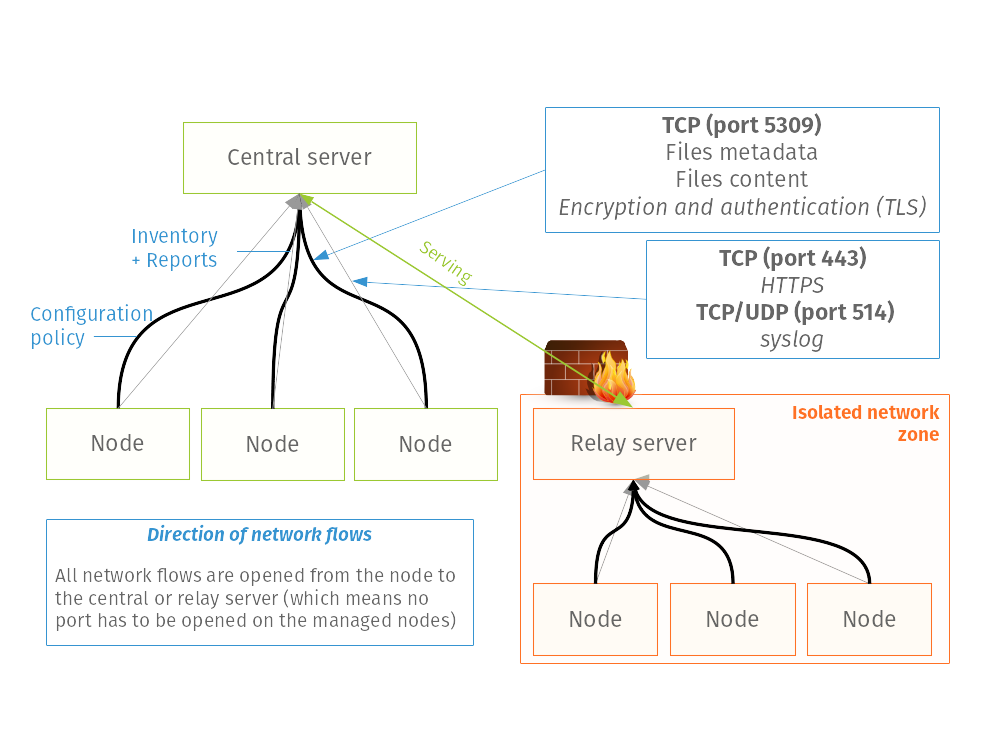
\includegraphics[scale=0.7]{network_connections.png}
		\end{center}
	\end{figure}
\end{frame}

\begin{frame}{Agent-server communication}

	\note{
	}
	\begin{itemize}
		\item HTTP PUT for inventories
		\item Custom protocol in TLS for policy copy
		\item Standard syslog for reporting
	\end{itemize}
\end{frame}

\begin{frame}[fragile]
	\note{
		This is what a report looks like.
		Every time the policies do something, we have to display a
		formatted report.

		It is actually hard to get reporting everywhere in the policies.
	}
	\begin{verbatim}
R: @@osquery_installation_and_configuration
@@result_success
@@32377fd7-02fd-43d0-aab7-28460a91347b
@@de4435a0-b5db-401a-aba1-a685d8a937e1
@@0
@@File from HTTP server
@@/etc/pki/RPM-GPG-KEY-osquery
@@2020-01-31 22:16:00+00:00
##2f4e4400-3206-4fb3-ae7f-16d1192e38ac
@#File /etc/pki/RPM-GPG-KEY-osquery is correct
\end{verbatim}
\end{frame}

\begin{frame}[fragile]{Reporting}

	\begin{verbatim}
R: @@Technique@@Type@@RuleId@@DirectiveId
@@VersionId@@Component@@Key@@ExecutionTimeStamp
##NodeId@#HumanReadableMessage
\end{verbatim}

	\begin{itemize}
		\item Produced by the policies (a lot of work actually!)
		\item One log in syslog for each component
		\item Special cases for the first and last report
		\item The webapp only processes them when last report is received
		      % 500 lines of awk, compatible, portable and... actually quite terrible
		\item Parsed using \texttt{awk} for \texttt{rudder agent run output}
	\end{itemize}
\end{frame}

\section{Needs and requirements}

\begin{frame}{Reporting - Current limitations}
	\begin{itemize}
		\item Reporting security
		      \begin{itemize}
			      \item plain text
			      \item no authentication (easy to fake)
		      \end{itemize}
		\item Missing information in reports
		      \begin{itemize}
			      \item Differences between expected and current state
			      \item Information about what has been repaired exactly
		      \end{itemize}
		\item Syslog itself
		      \begin{itemize}
			      \item Requires a specific port (514)
			      \item Requires root access (to configure local syslog daemon)
			      \item Can interact with user's syslog configuration
			      \item Hard to debug (not much logs about syslog daemon by default)
			      \item Poor performance (for database insertion)
		      \end{itemize}
	\end{itemize}
\end{frame}

\begin{frame}{Constraints}
	\note{
		Should be usable in production quickly.
		Should keep our "easy upgrades" contract.
	}
	\begin{itemize}
		\item Smooth transition
		      \begin{itemize}
			      \item Keep compatibility with both reporting modes for several versions
			      \item Allow switching at any time (same data model)
		      \end{itemize}
		\item \emph{Keep It Simple}
		      \begin{itemize}
			      \item Debuggable
			      \item Low operation overhead
			      \item Use well-known technologies
		      \end{itemize}
		\item Security
		      \begin{itemize}
			      \item State-of-the-art security for reporting protocol
			      \item Allow future homogenization
			      \item Focus on security for the implementation itself
		      \end{itemize}
	\end{itemize}
\end{frame}

\section{Design choices}

\begin{frame}{Report → Run log}
	\note{
		A run log is self contained (node id, config id, date), while reports were useless alone.
		Avoid meaningless situation (like 30\% of missing reports in a run)
	}

	\begin{itemize}
		\item The stream of reports is useless
		\item Better transmitted as a single run log
		\item Store information by run (in a simple file)
		\item Easier to manage and allows lots of improvements
		      \begin{itemize}
			      \item Compression (works well!)
			      \item Database transaction by run
		      \end{itemize}
		\item A run log is identified by: a node id, a config id and a date+time
	\end{itemize}
\end{frame}

\begin{frame}{Improve run log}

	\begin{itemize}
		\item We are missing a lot of valuable information
		\item "Hidden" in agent logs (\texttt{rudder agent run -i})
		\item Need to \texttt{ssh} to understand anything
		\item We want to capture and contextualize them
	\end{itemize}
\end{frame}


\begin{frame}
	\begin{figure}
		\begin{center}
			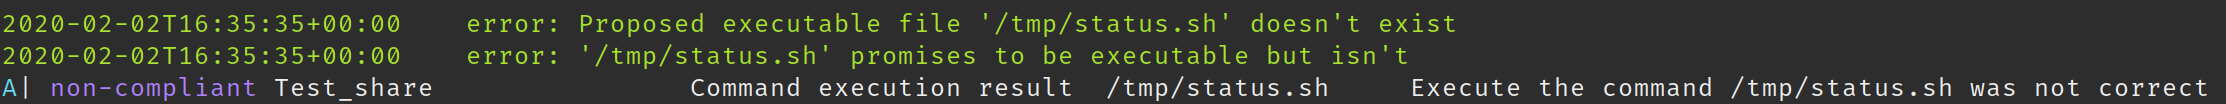
\includegraphics[width=400pt]{output.png}
		\end{center}
	\end{figure}
\end{frame}

\begin{frame}{Improve run log}

	The problem is that we have two (isolated) information streams:

	\begin{itemize}
		\item Reports from inside of the policies
		\item Agent logs (errors, executed commands, various outputs, etc)
	\end{itemize}
	

\end{frame}	
	\begin{frame}{Improve run log}
	\begin{itemize}
		\item Agents are usually not designed for error management at scale,
	and expect human interaction.
		\item Nothing built-in for automated outcome analysis (what failed and what has been done)
		      \begin{itemize}
			      \item no structured errors in the policies, only access to a state (\texttt{error/ok/repaired}) from inside the policy
			      \item no business knowledge in the logs
		      \end{itemize}
	\end{itemize}
\end{frame}

\begin{frame}[standout]
	\note{Not beautiful, but actionable today. "Low hanging fruit".
	Act as if we are human and provide our dream agent interface.}
	Use (=parse) \texttt{stdout}
\end{frame}

\begin{frame}{Improve run log}
	\begin{itemize}
		\item Capture full agent output in info mode
		\item Parse it on the relay/server
		\item Associate simple logs with following contextualized log
		\item Works for log from the technique editor or modern techniques
		\item Not that good for legacy techniques: do everything then report
		\item Specific insertion/purging configuration for non-results logs (=simple logs) 
	\end{itemize}
\end{frame}

\begin{frame}
	\begin{figure}
		\begin{center}
			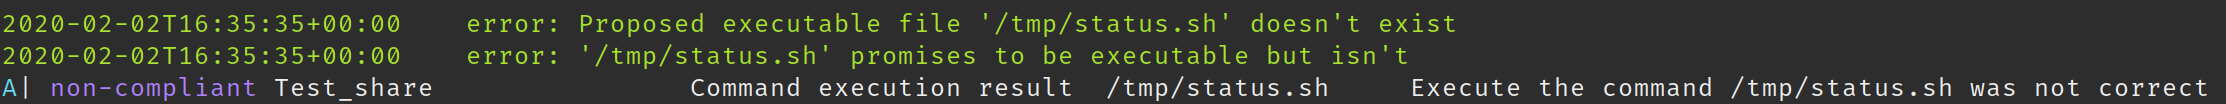
\includegraphics[width=400pt]{output.png}
		\end{center}
	\end{figure}
	\begin{figure}
		\begin{center}
			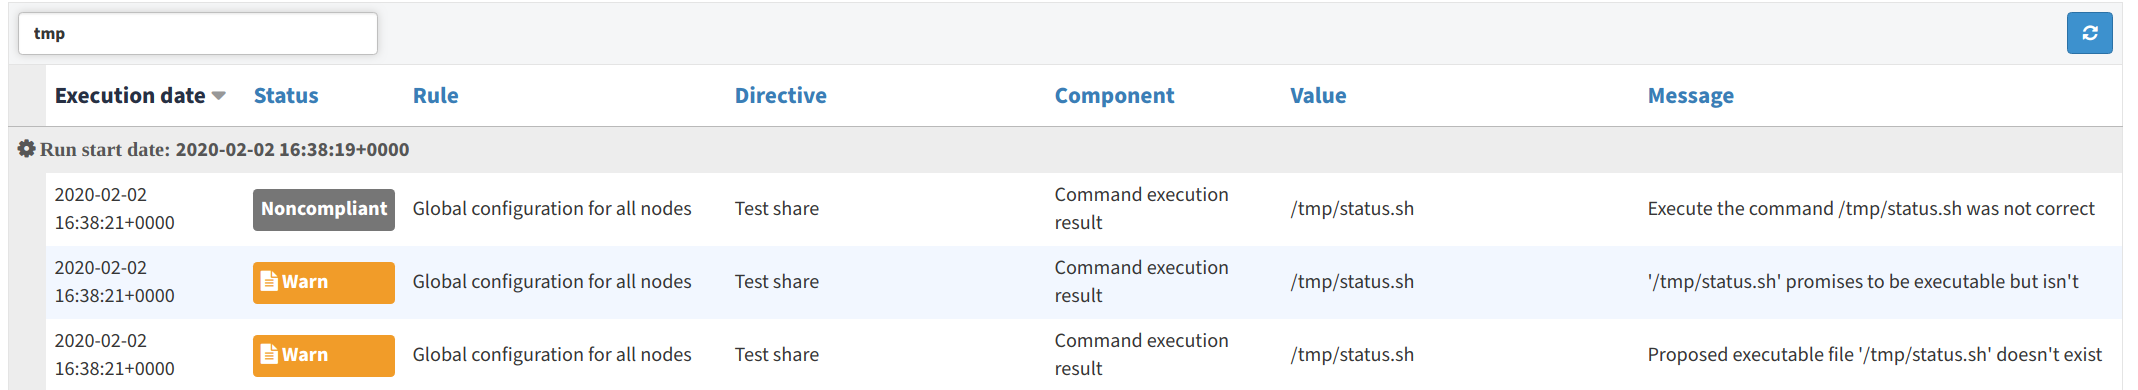
\includegraphics[width=400pt]{status.png}
		\end{center}
	\end{figure}
\end{frame}

\begin{frame}{Reports authentication}
	\begin{itemize}
		\item We want to authenticate reporting
		\item We want to stay asynchronous
	\end{itemize}
	
		\begin{itemize}
		\item End to end validation (check signature on root server)
		\item We need a signature (like we do for inventories)
		\item Prefer a standard
		\item We have a hierarchical node structure
	\end{itemize}
\end{frame}

\begin{frame}[standout]
	S/MIME
	\note{I know what you think. But it really suits our needs.}
\end{frame}

\begin{frame}{HTTP}
	Use HTTP as it's:
	\begin{itemize}
		\item Already used for inventories (and Windows policy downloads)
		\item Well-known
		\item Easy operation and debugging (curl, etc.)
		\item Fast and powerful enough (even more with HTTP/2)
		\item Use simple file PUT (like inventories)
	\end{itemize}
\end{frame}

\section{Implementation}

\begin{frame}{Agent}
	\begin{itemize}
		\item Use the existing \texttt{rudder agent run} wrapper
		\item Collect output, sign and compress
		\item Send to the server
		\item Retry in case of failure
		\item Allows back-filling compliance data
	\end{itemize}
\end{frame}

\begin{frame}{relayd}
	\begin{itemize}
		\item A new daemon that runs on all policy servers (root + relay)
		\item Reminder: A root server is also a relay
		\item Replaces relay python API
		\item Layer between the webapp and the nodes
		\item Stateless (except for history)
	\end{itemize}
\end{frame}

\begin{frame}{Relay API}
	\begin{itemize}
		\item Based on what existed since 3.2 (implemented in Python)
		\item Now versioned and documented
		\item Only listens locally
		\item Some endpoints behind \texttt{httpd} reverse proxy
		\item \href{https://docs.rudder.io/api/relay}{https://docs.rudder.io/api/relay}
		\item Still missing a full stats/monitoring API (prometheus?)
	\end{itemize}
\end{frame}

\begin{frame}{Relay API}
	\begin{itemize}
		\item \texttt{/system/\{status, reload, info\}}
		\item \texttt{/policies/\{node-id\}/rules}
		\item \texttt{/remote-run/nodes/\{id\}}
		\item \texttt{/shared-files/\{target-id\}/...}
		\item \texttt{/shared-folder/\{path\}}
	\end{itemize}
\end{frame}

\begin{frame}{relayd}
	\begin{itemize}
		\item Config files: \texttt{/opt/rudder/etc/relay}
		\item A new \texttt{rudder-relayd} service
		\item Logs to \texttt{journald}
		\item Part of the \texttt{rudder-server-relay} package
	\end{itemize}
\end{frame}

\begin{frame}[fragile]{Service hardening}

	\note{We have to use systemd, at least take advantage of the good parts (on compatible OSes)}

	\begin{verbatim}
User=rudder-relayd
ProtectSystem=strict
ReadWritePaths=/var/rudder/reports
    /var/rudder/inventories
    /var/rudder/shared-files
PrivateTmp=True
\end{verbatim}
\end{frame}

%\begin{frame}{Service hardening}
%Might add a seccomp filter later but a bit tricky on diverse platforms.
%\end{frame}

\begin{frame}[fragile]{SELinux}

	A dedicated SELinux context

	\begin{itemize}
		\item Write access to work directories
		\item Read access to configuration and data files
		\item Connect to HTTP and postgresql ports
		\item Listen on port 3030
		\item Run the `rudder remote run` command with sudo
	\end{itemize}

\end{frame}

\begin{frame}{HTTP security}
	\begin{itemize}
		\item Enforce TLS1.2+ everywhere (except syslog!)
		\item Option to check certificates in all HTTP requests
		\item Not directly linked
		\item Allows authentication of both ways
		\item For now, requires an existing PKI (and proper DNS setup)
	\end{itemize}
\end{frame}

\begin{frame}{Rust}

	\note{Embedded like in "Raspberry Pi". Bad experience with python.}

	\begin{itemize}
		\item We wanted:
		      \begin{itemize}
			      \item Reliability and security
			      \item Maintainability (<3 strong typing)
			      \item Low footprint (to allow "embedded" relayd)
			      \item Easy packaging and deployment
		      \end{itemize}
		\item Chose Rust!
	\end{itemize}
\end{frame}

\begin{frame}{To sum up}

We added a daemon between root server and nodes to:

	\begin{itemize}
	  \item Forward reports and inventories (inotify-based)
	  \item Check, parse and store reports on root server
	  \item Provide the file sharing API
	  \item Provide the policy and shared-files download API (for Windows)
	  \item Only required \texttt{httpd} and agent to synchronize data files
	\end{itemize}
\end{frame}

\section{Perspectives}

\begin{frame}{Future}
\note{The fist goal was to see ~ nothing!}
	\begin{itemize}
		\item Encryption option (using S/MIME)
		\item Use S/MIME for inventories too
		\item Allow policy updates over HTTPS for full HTTP communication
		      % This requires a bit of work but is definitely possible now
		\item Diffs for all non-compliance or errors (including files!)
		\item Connected mode for reactivity and continuity
		\item Flexible RUDDER server distribution (container, roles, cloud, etc)
		\item New (virtual) agents (maybe managed from relayd)
		\item Check server certificate by default
	\end{itemize}
\end{frame}

\begin{frame}[standout]
	Feedbacks?
	\note{Join us for dinner?}
\end{frame}

\begin{frame}[standout]
	Thank you!
\end{frame}

\end{document}
